\section*{Ejercicio 3}
\graphicspath{{Figuras/}}

En este ejercicio se busco obtener un histograma de la tasa de disparo dependiente del tiempo $r(t)$. Esta se obtiene calculando el promedio de spikes en las 128 realizaciones para cada intervalo de tiempo, en este caso $0.1\,\text{ms}$, y luego dividiendo por dicho intervalo. El resultado obtenido puede observarse en la Figura \ref{03:fig:rt}. 

\begin{figure}[h!]
    \centering
    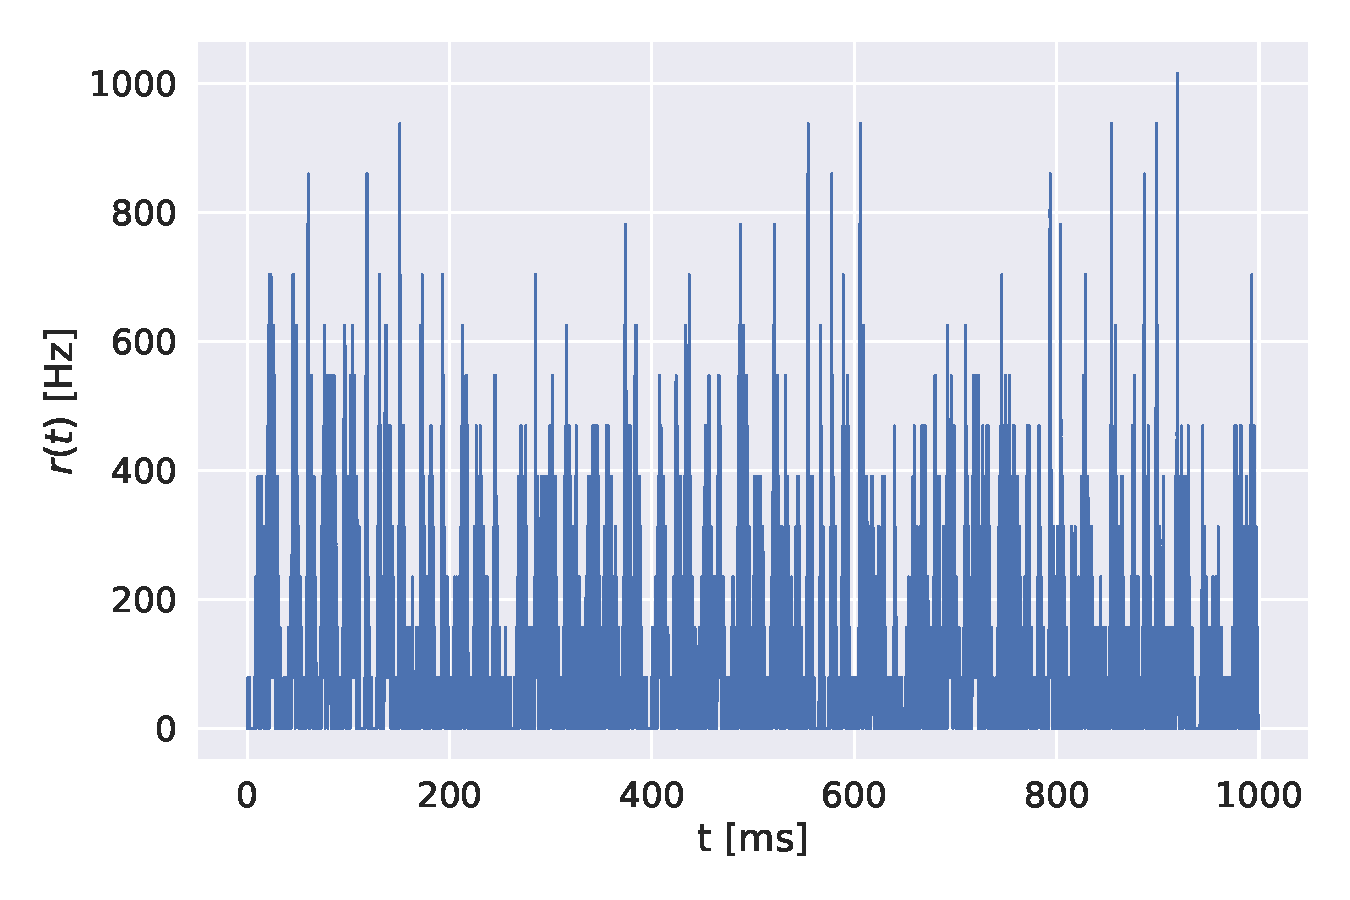
\includegraphics[width=0.75\textwidth]{3_rt.pdf}
    \caption{Histograma de la tasa de disparo $r(t)$ como función del tiempo, promediada para las 128 realizaciones.}
    \label{03:fig:rt}
\end{figure}